% Methodology
% Target: 2-3 pages

\subsection{Overview}
% TODO: Add system diagram figure
Our approach consists of three stages:
(1) Acoustic feature extraction from TTS-synthesized speech
(2) Emotion-augmented knowledge distillation
(3) Student model training with emotion embeddings

\subsection{Acoustic Feature Design}
\label{subsec:acoustic_features}

\subsubsection{Prosodic Features (13D)}
Based on emotion psychology literature \cite{TODO}:
\begin{itemize}
    \item \textbf{Pitch dynamics} (7D): mean, std, min, max, range, slope, variance
    \item \textbf{Energy} (3D): mean, std, max
    \item \textbf{Temporal} (3D): duration, speech rate, zero-crossing rate
\end{itemize}

\textbf{Rationale:} Prosody encodes emotional arousal and valence \cite{TODO}.

\subsubsection{Spectral Features (30D)}
Based on speech signal processing \cite{TODO}:
\begin{itemize}
    \item \textbf{MFCCs} (26D): 13 coefficients + delta coefficients
    \item \textbf{Spectral statistics} (4D): centroid, rolloff, flux, bandwidth
\end{itemize}

\textbf{Rationale:} Spectral envelope captures vocal tract configuration changes under emotion.

\subsubsection{Formant Features (3D)}
Based on acoustic phonetics \cite{TODO}:
\begin{itemize}
    \item F1, F2, F3 frequencies (voice quality indicators)
\end{itemize}

\textbf{Rationale:} Formants reflect vocal tract resonance affected by emotional state.

\subsection{Emotion-Augmented Architecture}
\label{subsec:architecture}

\subsubsection{Student Model}
Base: Qwen2.5-1.5B with LoRA adaptation
\begin{equation}
h_{\text{student}} = \text{LLM}(x; \theta_{\text{base}} + \Delta\theta_{\text{LoRA}})
\end{equation}

\subsubsection{Emotion Integration}
Concatenation-based fusion:
\begin{equation}
h_{\text{emotion}} = W_{\text{proj}} \cdot e_{\text{acoustic}}
\end{equation}
\begin{equation}
h_{\text{fused}} = [h_{\text{student}}; h_{\text{emotion}}]
\end{equation}

where $e_{\text{acoustic}} \in \mathbb{R}^{46}$ is the acoustic feature vector.

\subsubsection{Training Objective}
Language modeling loss:
\begin{equation}
\mathcal{L} = -\sum_{t=1}^{T} \log P(x_t | x_{<t}, e_{\text{acoustic}})
\end{equation}

\subsection{Baseline Comparisons}
\label{subsec:baselines}

\begin{itemize}
    \item \textbf{Text-Only}: No emotion features (baseline)
    \item \textbf{WavLM}: microsoft/wavlm-base-plus embeddings (256D)
    \item \textbf{Acoustic}: Our proposed features (46D)
    \item \textbf{Fusion}: Concatenation of WavLM + Acoustic (302D)
\end{itemize}

% TODO: Add architecture diagram
% \begin{figure}[t]
% \centering
% 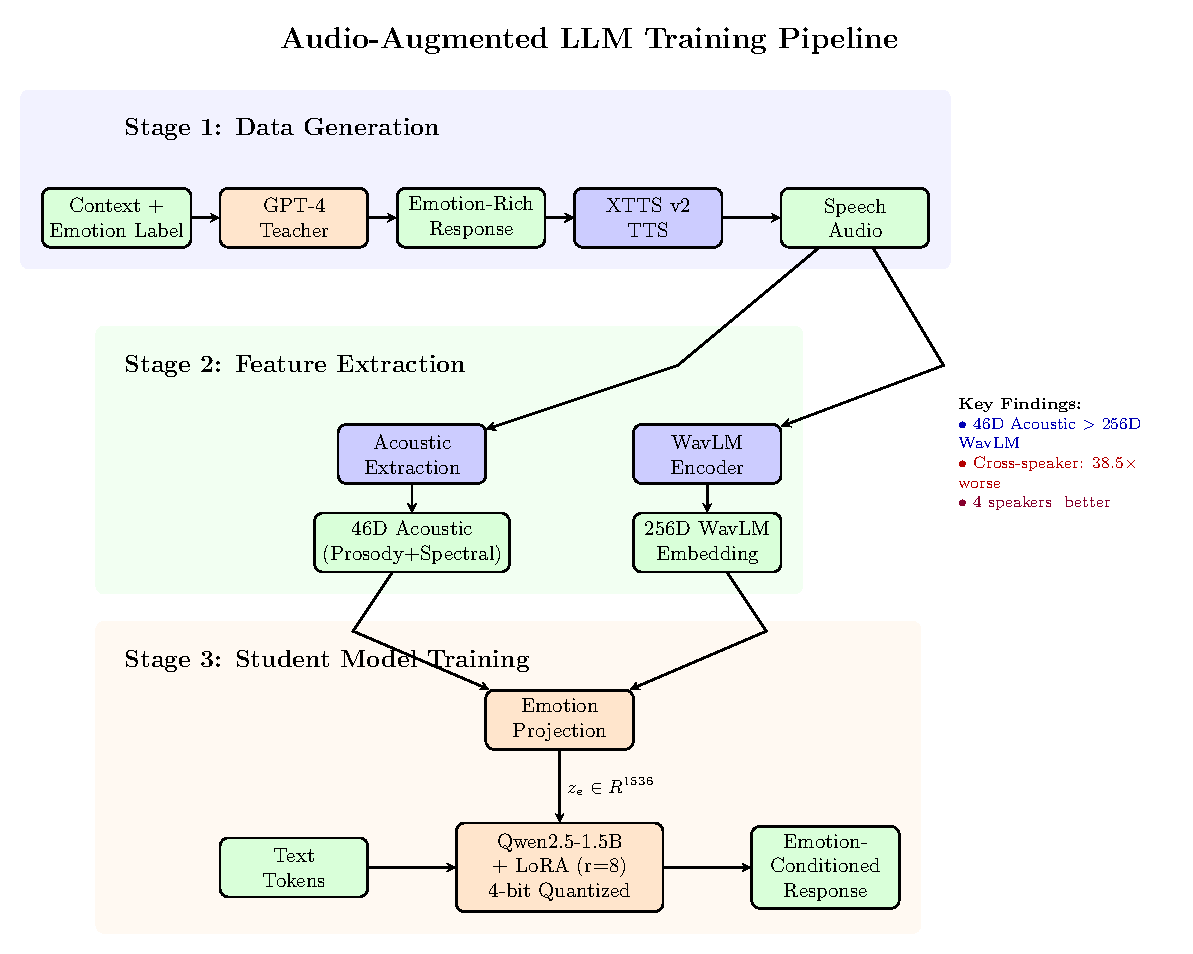
\includegraphics[width=0.48\textwidth]{figures/architecture.pdf}
% \caption{System architecture}
% \label{fig:architecture}
% \end{figure}
